% Created by tikzDevice version 0.12.3.1 on 2022-09-19 21:45:14
% !TEX encoding = UTF-8 Unicode
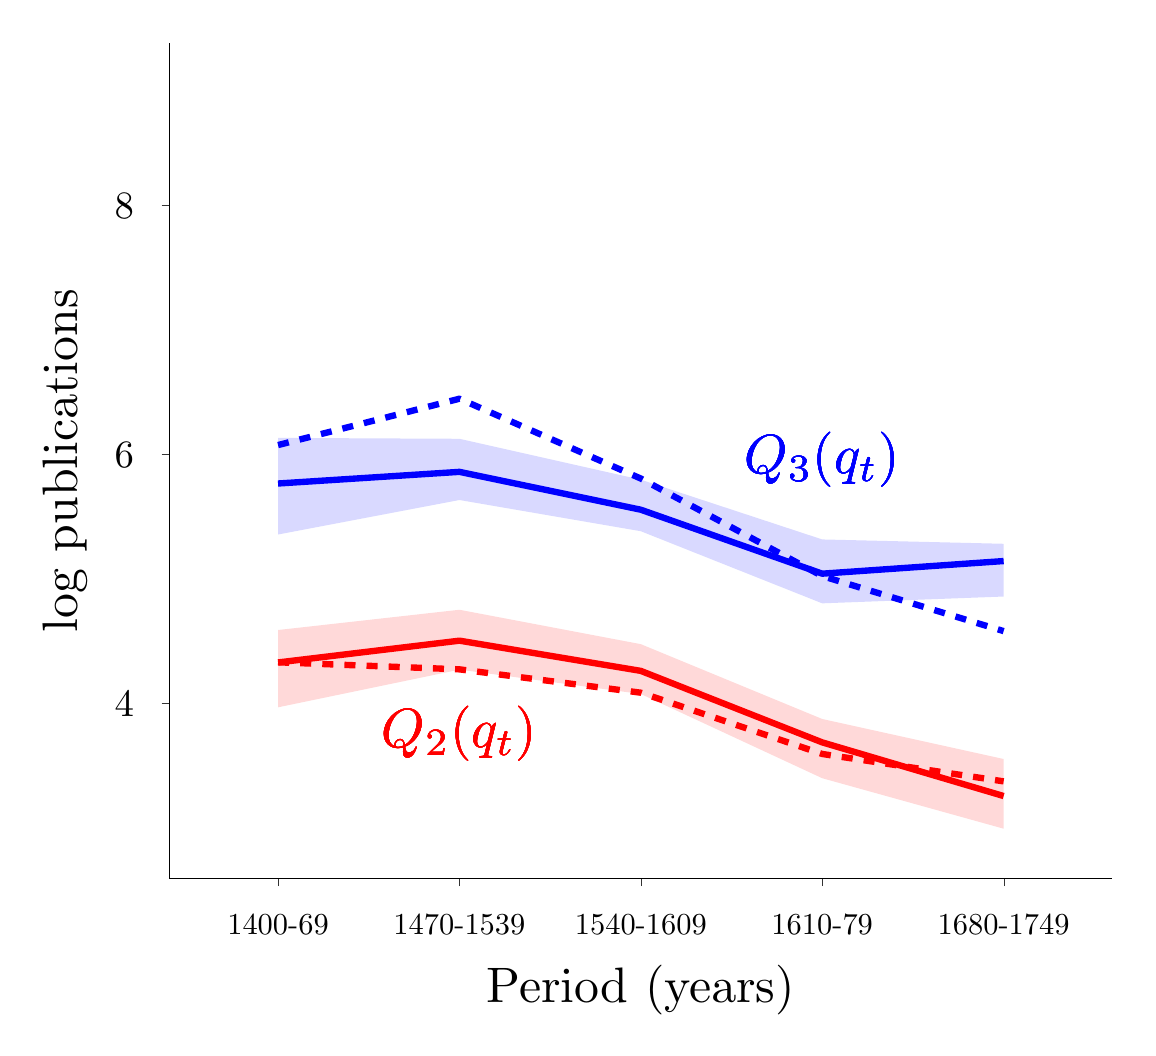
\begin{tikzpicture}[x=1pt,y=1pt]
\definecolor{fillColor}{RGB}{255,255,255}
\path[use as bounding box,fill=fillColor,fill opacity=0.00] (0,0) rectangle (397.48,361.35);
\begin{scope}
\path[clip] (  0.00,  0.00) rectangle (397.48,361.35);
\definecolor{drawColor}{RGB}{255,255,255}
\definecolor{fillColor}{RGB}{255,255,255}

\path[draw=drawColor,line width= 0.1pt,line join=round,line cap=round,fill=fillColor] (  0.00,  0.00) rectangle (397.48,361.35);
\end{scope}
\begin{scope}
\path[clip] ( 51.14, 53.86) rectangle (391.98,355.85);
\definecolor{fillColor}{RGB}{255,255,255}

\path[fill=fillColor] ( 51.14, 53.86) rectangle (391.98,355.85);
\definecolor{fillColor}{RGB}{255,0,0}

\path[fill=fillColor,fill opacity=0.15] ( 90.47,143.69) --
	(156.02,151.01) --
	(221.56,138.58) --
	(287.11,111.54) --
	(352.66, 97.08) --
	(352.66, 71.90) --
	(287.11, 90.14) --
	(221.56,120.58) --
	(156.02,129.37) --
	( 90.47,115.76) --
	cycle;

\path[] ( 90.47,143.69) --
	(156.02,151.01) --
	(221.56,138.58) --
	(287.11,111.54) --
	(352.66, 97.08);

\path[] (352.66, 71.90) --
	(287.11, 90.14) --
	(221.56,120.58) --
	(156.02,129.37) --
	( 90.47,115.76);
\definecolor{drawColor}{RGB}{255,0,0}

\path[draw=drawColor,line width= 2.3pt,line join=round] ( 90.47,131.97) --
	(156.02,139.84) --
	(221.56,128.92) --
	(287.11,103.09) --
	(352.66, 83.70);

\path[draw=drawColor,line width= 2.3pt,dash pattern=on 4pt off 4pt ,line join=round] ( 90.47,132.03) --
	(156.02,129.48) --
	(221.56,121.04) --
	(287.11, 98.90) --
	(352.66, 89.00);
\definecolor{fillColor}{RGB}{0,0,255}

\path[fill=fillColor,fill opacity=0.15] ( 90.47,213.11) --
	(156.02,212.79) --
	(221.56,198.01) --
	(287.11,176.42) --
	(352.66,174.85) --
	(352.66,155.79) --
	(287.11,153.33) --
	(221.56,179.39) --
	(156.02,190.67) --
	( 90.47,178.20) --
	cycle;

\path[] ( 90.47,213.11) --
	(156.02,212.79) --
	(221.56,198.01) --
	(287.11,176.42) --
	(352.66,174.85);

\path[] (352.66,155.79) --
	(287.11,153.33) --
	(221.56,179.39) --
	(156.02,190.67) --
	( 90.47,178.20);
\definecolor{drawColor}{RGB}{0,0,255}

\path[draw=drawColor,line width= 2.3pt,line join=round] ( 90.47,196.63) --
	(156.02,200.84) --
	(221.56,187.16) --
	(287.11,164.05) --
	(352.66,168.61);

\path[draw=drawColor,line width= 2.3pt,dash pattern=on 4pt off 4pt ,line join=round] ( 90.47,210.52) --
	(156.02,227.27) --
	(221.56,198.42) --
	(287.11,163.18) --
	(352.66,143.30);

\node[text=drawColor,anchor=base,inner sep=0pt, outer sep=0pt, scale=  1.99] at (287.11,200.25) {$Q_3(q_t)$};

\node[text=drawColor,anchor=base,inner sep=0pt, outer sep=0pt, scale=  1.99] at (287.11,200.25) {$Q_3(q_t)$};

\node[text=drawColor,anchor=base,inner sep=0pt, outer sep=0pt, scale=  1.99] at (287.11,200.25) {$Q_3(q_t)$};

\node[text=drawColor,anchor=base,inner sep=0pt, outer sep=0pt, scale=  1.99] at (287.11,200.25) {$Q_3(q_t)$};

\node[text=drawColor,anchor=base,inner sep=0pt, outer sep=0pt, scale=  1.99] at (287.11,200.25) {$Q_3(q_t)$};
\definecolor{drawColor}{RGB}{255,0,0}

\node[text=drawColor,anchor=base,inner sep=0pt, outer sep=0pt, scale=  1.99] at (156.02,101.23) {$Q_2(q_t)$};

\node[text=drawColor,anchor=base,inner sep=0pt, outer sep=0pt, scale=  1.99] at (156.02,101.23) {$Q_2(q_t)$};

\node[text=drawColor,anchor=base,inner sep=0pt, outer sep=0pt, scale=  1.99] at (156.02,101.23) {$Q_2(q_t)$};

\node[text=drawColor,anchor=base,inner sep=0pt, outer sep=0pt, scale=  1.99] at (156.02,101.23) {$Q_2(q_t)$};

\node[text=drawColor,anchor=base,inner sep=0pt, outer sep=0pt, scale=  1.99] at (156.02,101.23) {$Q_2(q_t)$};
\end{scope}
\begin{scope}
\path[clip] (  0.00,  0.00) rectangle (397.48,361.35);
\definecolor{drawColor}{RGB}{0,0,0}

\path[draw=drawColor,line width= 0.1pt,line join=round] ( 51.14, 53.86) --
	( 51.14,355.85);
\end{scope}
\begin{scope}
\path[clip] (  0.00,  0.00) rectangle (397.48,361.35);
\definecolor{drawColor}{RGB}{0,0,0}

\node[text=drawColor,anchor=base east,inner sep=0pt, outer sep=0pt, scale=  1.40] at ( 38.39,112.27) {4};

\node[text=drawColor,anchor=base east,inner sep=0pt, outer sep=0pt, scale=  1.40] at ( 38.39,202.28) {6};

\node[text=drawColor,anchor=base east,inner sep=0pt, outer sep=0pt, scale=  1.40] at ( 38.39,292.30) {8};
\end{scope}
\begin{scope}
\path[clip] (  0.00,  0.00) rectangle (397.48,361.35);
\definecolor{drawColor}{gray}{0.20}

\path[draw=drawColor,line width= 0.1pt,line join=round] ( 48.39,117.09) --
	( 51.14,117.09);

\path[draw=drawColor,line width= 0.1pt,line join=round] ( 48.39,207.11) --
	( 51.14,207.11);

\path[draw=drawColor,line width= 0.1pt,line join=round] ( 48.39,297.12) --
	( 51.14,297.12);
\end{scope}
\begin{scope}
\path[clip] (  0.00,  0.00) rectangle (397.48,361.35);
\definecolor{drawColor}{RGB}{0,0,0}

\path[draw=drawColor,line width= 0.1pt,line join=round] ( 51.14, 53.86) --
	(391.98, 53.86);
\end{scope}
\begin{scope}
\path[clip] (  0.00,  0.00) rectangle (397.48,361.35);
\definecolor{drawColor}{gray}{0.20}

\path[draw=drawColor,line width= 0.1pt,line join=round] ( 90.47, 51.11) --
	( 90.47, 53.86);

\path[draw=drawColor,line width= 0.1pt,line join=round] (156.02, 51.11) --
	(156.02, 53.86);

\path[draw=drawColor,line width= 0.1pt,line join=round] (221.56, 51.11) --
	(221.56, 53.86);

\path[draw=drawColor,line width= 0.1pt,line join=round] (287.11, 51.11) --
	(287.11, 53.86);

\path[draw=drawColor,line width= 0.1pt,line join=round] (352.66, 51.11) --
	(352.66, 53.86);
\end{scope}
\begin{scope}
\path[clip] (  0.00,  0.00) rectangle (397.48,361.35);
\definecolor{drawColor}{RGB}{0,0,0}

\node[text=drawColor,anchor=base,inner sep=0pt, outer sep=0pt, scale=  1.10] at ( 90.47, 33.53) {1400-69};

\node[text=drawColor,anchor=base,inner sep=0pt, outer sep=0pt, scale=  1.10] at (156.02, 33.53) {1470-1539};

\node[text=drawColor,anchor=base,inner sep=0pt, outer sep=0pt, scale=  1.10] at (221.56, 33.53) {1540-1609};

\node[text=drawColor,anchor=base,inner sep=0pt, outer sep=0pt, scale=  1.10] at (287.11, 33.53) {1610-79};

\node[text=drawColor,anchor=base,inner sep=0pt, outer sep=0pt, scale=  1.10] at (352.66, 33.53) {1680-1749};
\end{scope}
\begin{scope}
\path[clip] (  0.00,  0.00) rectangle (397.48,361.35);
\definecolor{drawColor}{RGB}{0,0,0}

\node[text=drawColor,anchor=base,inner sep=0pt, outer sep=0pt, scale=  1.80] at (221.56,  9.00) {Period (years)};
\end{scope}
\begin{scope}
\path[clip] (  0.00,  0.00) rectangle (397.48,361.35);
\definecolor{drawColor}{RGB}{0,0,0}

\node[text=drawColor,rotate= 90.00,anchor=base,inner sep=0pt, outer sep=0pt, scale=  1.80] at ( 17.90,204.86) {log publications};
\end{scope}
\end{tikzpicture}
